\documentclass[11pt, letterpaper, titlepage]{article}
\usepackage[utf8]{inputenc}
\usepackage{hyperref}
\hypersetup{pdfborder=0 0 0}
\usepackage{amsmath}
\usepackage{amssymb}
\usepackage{geometry}
\usepackage[none]{hyphenat}
\usepackage{xcolor}
\usepackage{cite}
\usepackage{lipsum}
\usepackage{physics}
\usepackage{textgreek}
\usepackage{unicode-math}
\usepackage{subfigure}
\usepackage{graphicx}
\usepackage{textgreek}
\usepackage{xcolor}
\geometry{
 a4paper,
 left=25mm,%left=20mm,
 right=25mm,%right=20mm,
 bottom=25mm, %bottom=20mm,
 top=25mm,%top=20mm,
 }

%%%%%%%% PORTADA
\title{
 \textbf{\LARGE UNIVERSITY OF OSLO} \\
\vspace{37mm}
\textbf{\Large Project report title}\\
\vspace{7mm}
\Large Special Curriculum \\
\vspace{25mm}
} 
\author{\Large Hishem Kløvnes \\ \textcolor{blue}{\href{https://github.com/hishemok/Special_curriculum}{GitHub Link} }} 
\date{\Large \today} % Deadline


\begin{document}
\sloppy
\maketitle
% \tableofcontents
\newpage



\Large Temporary report structure
\Large TODO: Fix citations and references
\section{Introduction}
% Quick introduction of the promise of quantum computing and the major hurdle of decoherence. This is where I introduce topological quantum computation as a potential solution, highlighting its reliance on non-local, protected qubits. 
% \par
% \textbf{Goal:} Realizing MZMs\\
% \textbf{Challenge:} Mention the top-down approach using nanowires and its experimental difficulties (notes from note section 5.1)\\
% \textbf{Alternative:} Introduce the bottom-up approach QD-SC-QD systems to create a minimal, highly tunable Kitaev chain. Define the concept of PMMs. \\
% \textbf{Research Question:} Objective: "This report will provide the theoretical background for superconductivity in hybrid systems and present an analytical and numerical investigation into the emergence and robustness of PMMs in a double QD system". \\
% \textbf{Draft:}\\
Superconductivity, as described by Bardeen-Cooper-Schrieffer (BCS) theory, arises from the formation of Cooper pairs. These are bound pair of electrons with opposite momentum and spin. The pairing leads to an energy gap in the excitation spectrum, which protects the superconducting state from low-energy perturbations. Whem superconductivity is induced in hybrid systems, such as semiconductor proximitized by superconductors, it can give rise to emergent quasiparticle excitations with exotic properties. Majorana zero modes, are one such excitation that can appear at the ends of one-dimensional topological superconductors. These modes are predicted to obey non-Abelian exchange statistics, which makes them suitable for fault-tolerant quantum computation, meaning: information is stored in the joint parity of spatially separated modes, rendering it insesitive to local perturbations.\\ \\
To identify and manipulate MZMs, it is important to examine their non-local nature and the conditions under which they arise. The quantum information encoded in these modes is associated with fermionic parity rather than local charge, motivating measurements that distinguish between even and odd parity ground states without collapsing the non-local encoding. This conceptual framework directly informs the design and interpretation of experiments in minimal realizations of Majorana systems, where one seeks to reproduce the essential physics in a controlable, highly tunable setup. \\ \\
In this report, we investigate the Poor Man's Majoranas (PMMs) in a double quantum dot-suprcondcutor-quantum dot (QD-SC-QD) system. PMMs provide a bottom-up, minimal Kitaev chain realization, capturing the key features of MZMs while remaining experimentally accessible and numerically tractable. By combining analytical and numerical approaches, we explore the emergence of zero-energy modes, their spatial localization, and the robustness of their degeneracy under variations in system parameters, providing insight into the feasiblity of realizing topologically protected qubits in such minimal systems.\\


















\section{Theoretical Background: The superconducting State}
Notes from note section 1 and note section 2 to build necessary background.\par
\subsection{From Electron Attraction to the Energy Gap:} 
Superconductivity is characterized by the complete loss of electrical resistance below a critical temperature $T_c$, and the expulsion of magnetic fields (the Meissner effect), which demonstrates that it represents a distinct thermodynamic phase rather than a perfect conductor.\\
Londong (1937) first introduced a phenomenological description in terms of a macroscopic quantum wavefunction $ψ(r)$, whose rigidity gives rise to the London equations and an exponential decay of magnetic fields inside the superconductor over a characteristic length scale, the London penetration depth $λ_L = \sqrt{m / (μ_{0}e² |ψ|²)}$ \textcolor{red}{CITATION}[CambridgeBCS.pdf chapter 2].\\
Microscopically, the origin of superconductivity lies in an effective attraction between electrons mediated by lattice vibrations (phonons). This leads to the formation of Cooper pairs, which are bound states of two electrons with opposite momenta and spins. The exchange of a virtual phonon leads to an attractive interaction for energy transfers smaller than the phonon frequency $ω_D$,
$$
V_{eff}(q,ω) = \frac{|g_q|²}{ω² - ω_q²} 
$$
where $g_q$ is the electron-phonon coupling strength zand $ω = (ϵ_k - ϵ_k')$, and the $ϵ_α$ are the single-particle energies. The isotope effect, where $T_c$ varies inversely with the square root of the ionic mass, provides strong evidence for the phonon-mediated pairing mechanism.\textcolor{red}{CITATION}[CambridgeBCS.pdf chapter 3].\\
In his seminal work, Cooper (1956) demonstrated that an arbitrarily weak attractive interaction destabilizes the Fermi sea: two eelectrons of opposite spin and momentum can form a bound state with energy below the Fermi level. The pair is called a Cooper pair, and the operator we use to describe the creation of a Cooper pair is;
$$
Λ^{†} = ∑_{k}^{}ϕ(k) c_{k↑}^{†} c_{-k↓}^{†} 
$$
and the self-consistency condition 
$$
1 = g_{0} N(0) ∫_{0}^{ω_D} \frac{dϵ}{\sqrt{2ϵ² + E}}
$$
yields the binding energy of the Cooper pair:
$$
E_B = -2ω_D e^{-2/(g_0 N(0))}
$$
where $N(0)$ is the density of states at the Fermi level and $g_0$ is the effective interaction strength \textcolor{red}{CITATION}[CambridgeBCS.pdf chapter 3.2 and BCS.pdf]\\ 
Even this simple two-particle result implies that the Fermi surface is unstable toward pair condensation.\\ \\
Building on Cooper's insight, Bardeen, Cooper, and Schrieffer (1957) developed a comprehensive microscopic theory of superconductivity \textcolor{red}{CITATION}[BCS.pdf].\\. The VCS ground state is a coherent superpositon of occupied and unoccupied pair states:
$$
\ket{Ψ_{BCS}} = ∏_{k} (u_k + v_k c_{k↑}^{†} c_{-k↓}^{†}) \ket{0}
$$
with normalization $|u_k|² + |v_k|² = 1$. Minimization of the free energy yields the gap equation:
$$
1 = \frac{g_0}{V} ∑_{|ϵ_k| < ω_D}^{} \frac{1}{2E_k} \tanh\left(\frac{E_k}{2k_B T}\right)
$$
where the quasiparticle excitation spectrum is:
$$
E_k = \sqrt{ϵ_k² + Δ²}
$$
At zero temperature, the gap at the Fermi surface is:
$$
Δ(0) = 2ω_D e^{-1/(g_0 N(0))}
$$
and obeys the universal relation $2Δ(0) / k_B T_c ≈ 3.53$.\\
The energy gap $Δ$ represents the minimum energy required to break a Cooper pair, explainingt he exponential suppression of heat capacity and resistivity at low temperatures. Physically, it quantifies the rigidity of the condensate. Any single-particle excitation costs a funite energy, enforcing long-range phase coherence.\\
Superconducting excitations are Bogoliubov quasiparticles, coherent superpositions of electron and hole states, which naturally leads to the Bogoliubov-de Gennes (BdG) formalism. This formalism genereralizes the BCS mean-field theory to spatially inhomogeneous systems and forms the basis for the study of superconducting heterostructures, including those hosting Majorana modes.\\


\subsection{The Bogoliubov-de Gennes Formalism:}
The microscopic BCS theory descirbes superconductivity as a coherent condensate of Cooper pairs, but it assumes a uniform order parameter $Δ$. To describe spatially varying superconducting states, such as those at interfaces or in the presence of impurities, we must generalize the BCS mean-field Hamiltonian to include position dependence. This leads us to the Bogoliubov-de Gennes (BdG) formalism \textcolor{red}{CITATION}[CambridgeBCS.pdf chapter 14 and BCS.pdf].\\
Starting from the BCS mean-field Hamiltonian,
$$
H_{MF} = ∫ d³r \left[ ∑_{σ} ψ_{σ}^{†}(r) H_0 ψ_{σ}(r) + (Δ(r) ψ_{↑}^{†}(r) ψ_{↓}^{†}(r) + h.c.) \right]
$$
where $H_0 = \frac{p²}{2m}-μ + V(r)$ describes the normal-state single particle dynamics, and $Δ(r)$ is the superconducting pair potential. We can diagonalize this Hamiltonian by introducing Bogoliubov  through canonical transformations:
$$
ψ_{↑}(r) = ∑_{n} [u_n(r) γ_{n↑} - v_n^{*}(r) γ_{n↓}^{†}], \quad ψ_{↓}(r) = ∑_{n} [u_n(r) γ_{n↓} + v_n^{*}(r) γ_{n↑}^{†}]
$$
Substituting and deminding that the quasiparticle operators $γ_{nσ}$ diagonalize the Hamiltonian leads to the BdG equations:
$$
\begin{pmatrix}
H_0(r) & Δ(r) \\
Δ^{*}(r) & -H_0^{*}(r)
\end{pmatrix}
\begin{pmatrix}
u_n(r) \\
v_n(r)
\end{pmatrix}= E_n
\begin{pmatrix}
u_n(r) \\
v_n(r)
\end{pmatrix}
$$
Each eigenstate ($u_n(r), v_n(r)$) represents a Bogoliubov quasiparticle, a coherent superposition of electron and hole amplitudes. The corresponding excitation energies $E_n ≥ 0$ define the superconducting quasiparticle spectrum.\\
Because both particle hole components are included, the BdG Hamiltonain possesses an intrinsic particle-hole symmetry. 
$$
Ξ H_{BdG} Ξ^{-1} = -H_{BdG}, \quad Ξ = τ_x K
$$
where $τ_x$ acts in particle-hole space and $K$ is complex conjugation. This symmetry enforces that the spectrum is symmetric about zero energy: if $E_n$ is an eigenvalue, so is $-E_n$.\\
This doubling of the Hilbert space is not redundant, it reflects the physical reality that the superconducting condensate does not conserve particle number, but rather fermion parity. The eigenstates at $± E_n$ correspond to the same physical excitation, and a zero-energy solution ($E_n = 0$) indicates a self-conjugate quasiparticle, $γ = γ^{†}$, which is the defining property of a Majorana mode\textcolor{red}{CITATION}[Topocondmat.org].\\
The BdG framework therefor bridges microscopic BCS theory and modern topological superconductivity. It provides a compact description of inhomogeneous superconductors, quantum dots coupled to superconducting leads, and low dimensional systems where topological phases can emerge.

\subsection{Hybrid Systems and the Proximity Effect:} 
The proximity effect is a phenomenon where a semiconductor acquires superconducting correlations when placed in contact with a superconductor. This mechanism is central to modern hybrid quantum devices and enables the creation of exotic quantum states, such as topological superconductivity, from conventional materials. This strategy is often called a "top-down" approach, as it builds complex states from well-understood components.
\subsubsection{Induced pairing and the effective gap}
At the microscopic level, the superconductor hosts a condensate of Cooper pairs described by a pairing potential $Δ$. When a semiconductor is coupled to the SC throguh a transparent interface, Cooper pairs can leak into the semiconductor through virtual tunneling process. From the semiconductor's perspective, this induces an effective pairing amplitude $Δ_{ind}$, giving rise to the Bogoliubov quasiparticles with the spectrum:
$$
E_k = \sqrt{ϵ_k² + |Δ_{ind}|²}
$$
The semiconductor thereby becomes proximitized, it behaves as if it were superconducting, even though no intrinsic exists in the semiconductor itself. \textcolor{red}{CITATION}[Qtech].\\
The magnitude of the induced gap $Δ_{ind}$ depends on 
the parent gap $Δ$, interface transparency, tunneling coupling strength, and the relative densities of states in the SC and SM. To reach the topological regime, three effects must be carefully balanced:
\begin{itemize}
  \item S-Wave proximity coupling: Establishing a robust induced gap $Δ_{ind}$ and providing superconducting correlations in the semiconductor.
  \item Zeeman energy, $E_Z = \frac{1}{2} g μ_B B$, from applied magnetic field that tends to polarize spins and close the gap. 
  \item Spin-orbit coupling (SOC), which counteracts full spin alignment and preserves pairing correlations under magnetic fields.
\end{itemize} 
A topological phase occurs when the Zeeman energy mathes the cost associated with $Δ_{ind}$ and the chemical potential $μ$:
$$
E_Z = \sqrt{Δ_{ind}² + μ²}
$$
Above the critical field, the proximitized semiconductor behaves effectively as a spinless p-wave superconductor,  mathematically equivalent to the Kitaev chain. \textcolor{red}{CITATION}[Qtech].\\
Experimentally, realizing this regime requires a semiconductor with a large $g$-factor, low carrier density, and strong spin–orbit coupling. These conditions ensure a sizable induced gap and a stable topological phase without quenching the parent superconductivity.
\subsubsection{Andreev Reflection and Cooper-pair splitting}
At the SM–SC interface, subgap transport is governed by Andreev reflection (AR). When an electron from the SM with energy $|E|<\Delta$ impinges on the interface, it cannot enter the SC as a single quasiparticle. Instead, it is retro-reflected as a hole while a Cooper pair is transferred into the superconducting condensate \textcolor{red}{CITATION}[Qtech]\\
A nonlocal version, known as Crossed Andreev Reflection (CAR) or Cooper-pair splitting, occurs when the two electrons of a Cooper pair tunnel into spatially separated regions—e.g. into two distinct quantum dots (QDs) coupled via a central SC. This process dominates when the separation is shorter than the superconducting coherence length $\xi$.\\
In double-dot hybrid systems (QD–SC–QD), two tunneling processes compete \cite{qtech_boka}:
\begin{itemize}
  \item Local Andreev Reflection (LAR): Both electrons of a Cooper pair enter the same QD. This process is suppressed by the on-site Coulomb energy $U$, which disfavors double occupancy.
  \item Crossed Andreev Reflection (CAR): Each electron enters a different QD, bypassing the charging penalty and becoming the dominant Andreev process.
\end{itemize}
CAR provides a nonlocal pairing amplitude ($\Delta$) that directly maps onto the p-wave term in the minimal Kitaev chain, while Elastic Cotunneling (ECT) provides the effective hopping ($t$) between sites. The sweet-spot condition $|t|=|\Delta|$ marks the parameter regime where the two Majorana-like modes become spatially separated—the so-called poor-man’s Majorana limit \textcolor{red}{CITATION}[Qtech]\\
The CAR strength can be inferred experimentally from nonlocal current correlations. Under resonance ($\epsilon_L=-\epsilon_R$) the current from Cooper-pair splitting follows approximately
$$ I_{CAR} = \frac{e}{\bar{h}} \frac{Γ}{(ϵ_L + ϵ_R)^2 + Γ²} |Δ|²$$
where $\Gamma$ quantifies coupling to the leads. Measuring $I_{\mathrm{CAR}}$ and $I_{\mathrm{ECT}}$ thus allows tuning of hybrid dots to the Majorana regime.
\subsubsection{Andreev Bound States (ABS)}
Repeated Andreev reflections at confined interfaces give rise to discrete Andreev bound states (ABS) inside the superconducting gap ($|E|<\Delta$). ABS are coherent superpositions of electron and hole components, characterized by Bogoliubov amplitudes $(u,v)$. Their energies depend on gate-defined confinement and magnetic field, and they can transition from being even-parity (singlet-like) to odd-parity (doublet-like) as parameters vary.\\
In the QD–SC–QD architecture, ABS form the fundamental subgap excitations mediating CAR and ECT. Parity crossings in these ABS—visible as zero-energy crossings—signal a change in fermion parity and mark the precursor to Majorana physics in more extended structures \textcolor{red}{CITATION}[Qtech].

























\section{Engineering Majorana Modes in a Minimal System}
% Connect general theory to specific PMM platform, notes note section 4 and note section 5.2\par
\subsection{The Kitaev Chain Model}
We now want to build on the microscopic understanding of superconductivity we investigated in the previous sections. In particular, we want to see how such pairing phenomena can be engineered to host topological excitations, in particular, Majorana bound states. The theoretical foundation for this lies in the Kitaev chain model, a one-dimensional toy model that captures the essential ingredients of topological superconductivity in its simplest form \textcolor{red}{CITATION}[Topocondmat.org].\\
\begin{figure}
  \centering
  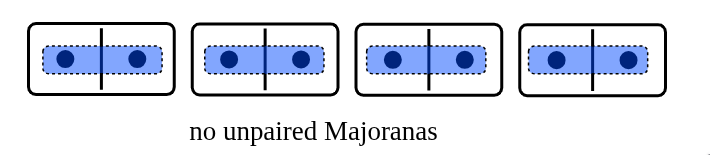
\includegraphics[width=0.45\textwidth]{../External_Figs/no_unpaired.png}
  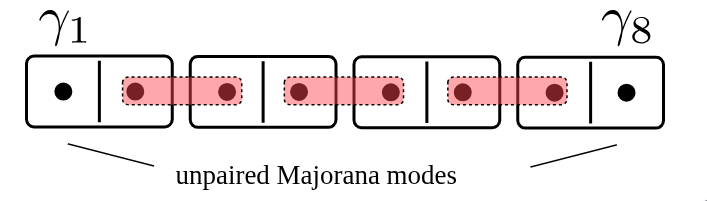
\includegraphics[width=0.45\textwidth]{../External_Figs/unpaired.png}
  \caption{Schematic representation of the Kitaev chain in its two distinct phases. Left: In the trivial phase, Majorana modes on the same site pair to form conventional fermions, leaving no unpaired modes. Right: In the topological phase, Majoranas on adjacent sites couple, leaving unpaired modes at the chain ends, which combine into a non-local fermionic mode. \textcolor{red}{CITATION}Topocondmat.org (Bulk edge correspondence in Kitaev chains)}
  \label{fig:kitaev}
\end{figure}
In the figure above \ref{fig:kitaev}, we see a schematic representation of the Kitaev chain in its two distinct phases, the trivial phase on the left and the topological phase on the right.\\
In the trivial phase, the Majorana modes on the same site pair to form conventional fermions, leaving no unpaired modes. In contrast, in the topological phase, Majoranas on adjacent sites couple, leaving unpaired modes at the chain ends, which combine into a non-local fermionic mode. At first glance, it may seem impossible to isolate a single Majorana mode, since condensed matter systems are composed of electrons, which always correspond to pairs of Majoranas. However, it turns out that by engineering the Hamiltonian appropriately, one can create a situation where two Majorana modes localize at opposite ends of a one-dimensional system, effectively separating them spatially. This separation is crucial for their non-Abelian statistics and potential applications in topological quantum computing\textcolor{red}{CITATION}[Topocondmat].\\
The Hamiltonian of the Kitaev chain is given by:
\begin{equation}
H = -\mu \sum_{j=1}^{N} \left(c_j^\dagger c_j - \frac{1}{2}\right)
- t \sum_{j=1}^{N-1} \left(c_j^\dagger c_{j+1} + c_{j+1}^\dagger c_j\right)
+ \Delta \sum_{j=1}^{N-1} \left(c_j c_{j+1} + c_{j+1}^\dagger c_j^\dagger\right),
\label{eq:kitaev_ham}
\end{equation}
where $μ$ is the chemical potential, or onsite energy, $t$ is the hopping amplitude, and $Δ$ is the p-wave pairing amplitude. The fermionic operators $c_j^\dagger$ and $c_j$ create and annihilate an electron at site $j$, respectively.\\
With the parameters $t=Δ=0$ and $μ ≠ 0$, the system is in a trivial insulating phase with no special edge states. However, tuning the parameters such that $t = Δ > 0$ and $μ = 0$, the edges become isolated, leaving two unpaired Majorana modes localized at the ends. These modes combine into a single non-local fermionic mode that costs zero energy to occupy. We will later explore how this model maps onto the QD–SC–QD system, and how the parameters can be tuned experimentally to reach this regime. 


\subsubsection{Bulk spectrum and topological phases}
To understand when the Kitaev chain supports topologically non-trivial states, we now turn from the real-space picture to its bulk description in momentum space. This transformation allows us to analyze the quasiparticle excitation spectrum and identify the conditions under which the superconducting gap closes and reopens.\\
Using translation invariance, we apply a Fourier transform,
$$
c_j = \frac{1}{\sqrt{N}} \sum_p e^{ipaj} c_p,
$$
This allows us to write the Hamiltonian (\ref{eq:kitaev_ham}) in momentum space $p$ as:
\begin{equation}
H = ∑_{ p}^{} ξ_p\left(c_p^{†} c_p - \frac{1}{2}\right) - ∑_{p}^{} t \cos p a + Δ ∑_{p}^{}\left(c_p^{†} c_{-p}^{†} e^{ipa} + c_{-p} c_p e^{-ipa}\right), 
\end{equation}
with $ξ_p = -μ - 2t \cos pa$ and $a$ the lattice spacing. This Hamiltonian becomes diagonal in the Bogoliubov–de Gennes (BdG) formalism. The resulting quasiparticle energy spectrum is:
\begin{equation}
  E_{p,\pm} = \pm \sqrt{(μ - 2t \cos{pa})^2 + 4Δ^2 \sin^2{pa}},
\end{equation}
The spectrum is gapped for most parameter values, but the gap closes when
$$
|μ| = 2|t|
$$
This marks the critical point separating two distinct superconducting phases. When $μ$ crosses this boundary, the system undergoes a topological phase transition: the character of the ground state changes without any symmetry breaking, but through a change in the topology of the quasiparticle band structure.\\
\begin{figure}
  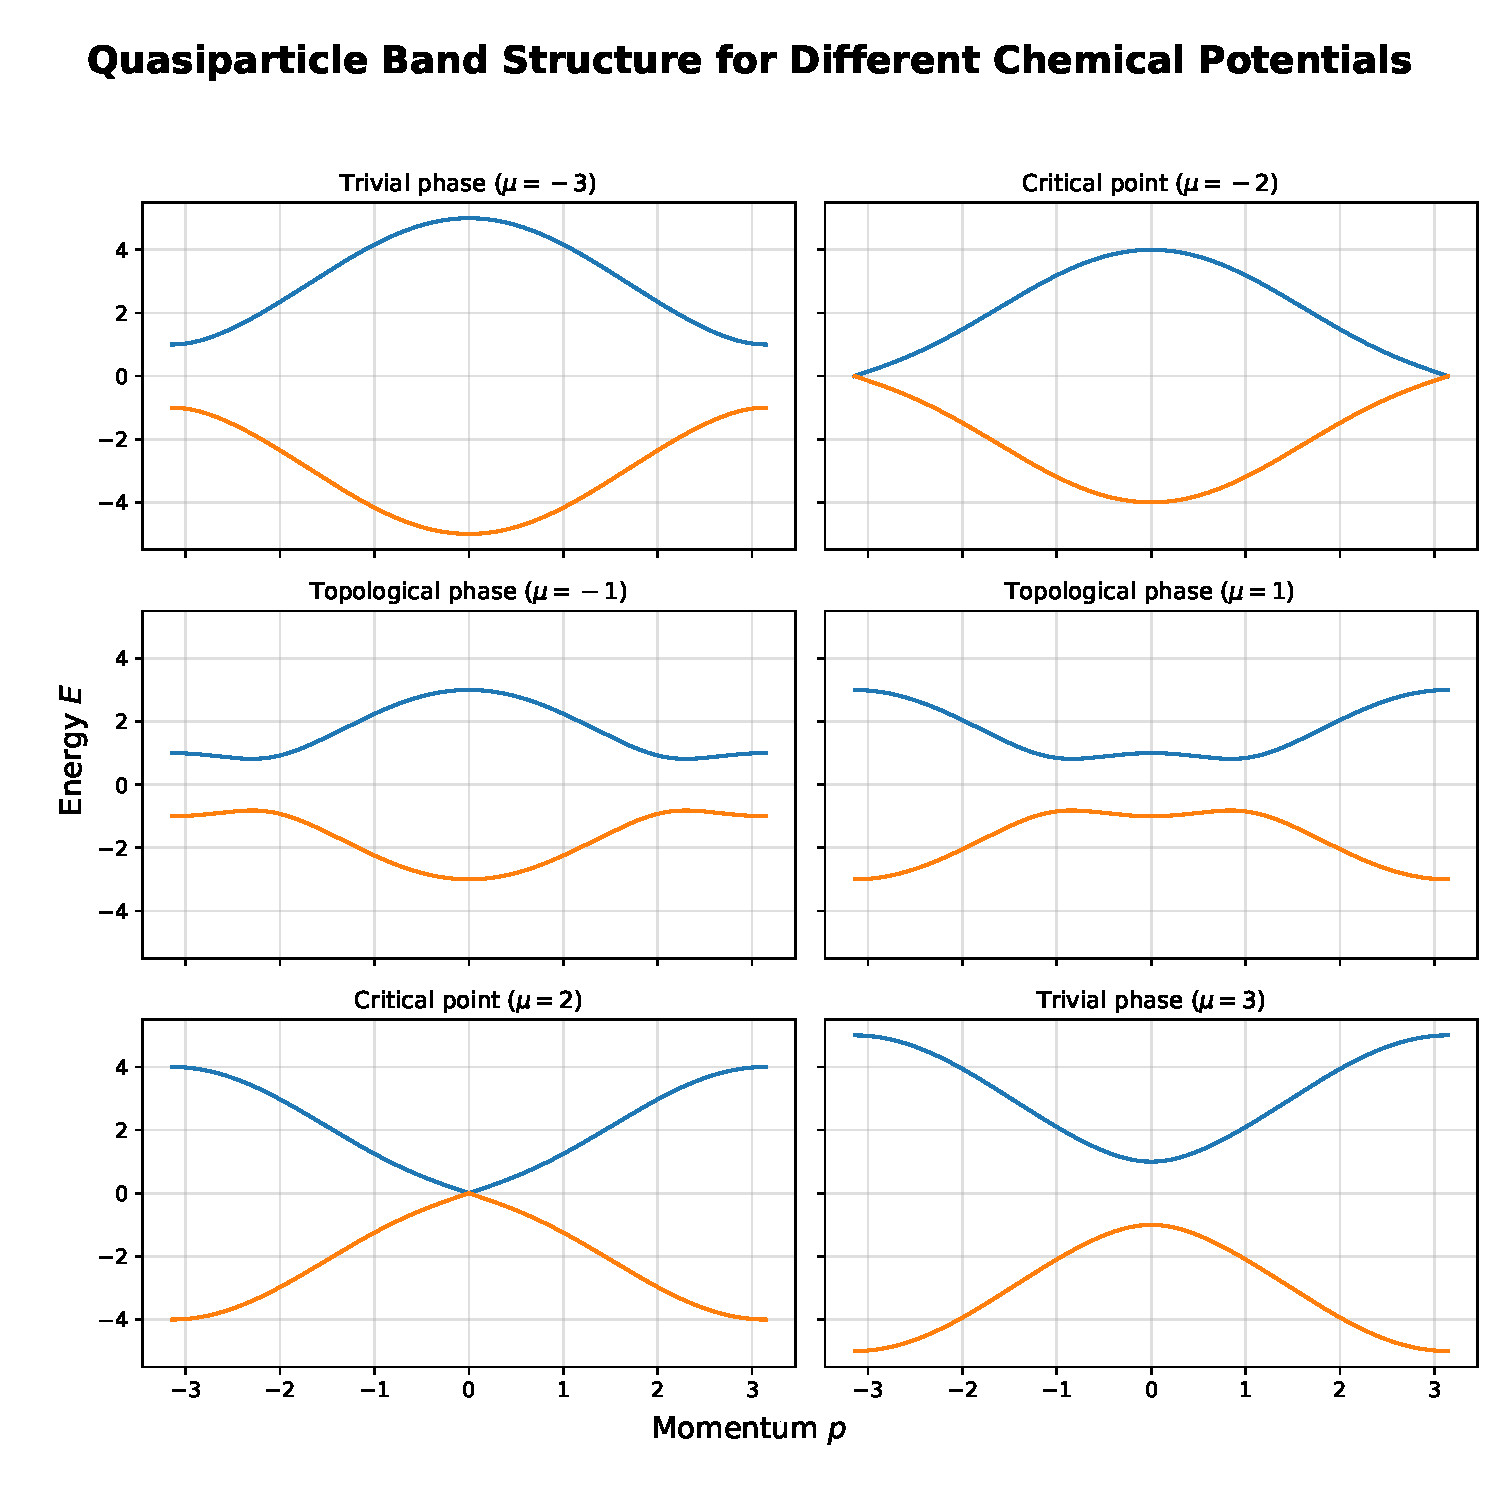
\includegraphics[width=1\textwidth]{../Figures/band_structure.pdf}
  \caption{Quasiparticle energy spectrum of the Kitaev chain for different chemical potentials $μ$. Left: In the trivial phase ($|μ| > 2|t|$), the spectrum is fully gapped with no zero-energy modes. Right: In the topological phase ($|μ| < 2|t|$), the gap closes and reopens, signaling the emergence of zero-energy edge modes.}
\end{figure}
\newpage


\subsubsection{Majorana representation and zero modes}
In order to further understand the nature of these boundry states, we can express each fermionic operator in terms of two real Majorana operators:
\begin{equation}
c_j = \frac{1}{2}(\gamma_j^A + i\gamma_j^B), \quad
c_j^\dagger = \frac{1}{2}(\gamma_j^A - i\gamma_j^B),
\end{equation}
where $\gamma_j^{A,B}$ satisfy $\{\gamma_j^\alpha, \gamma_k^\beta\} = 2\delta_{jk}\delta_{\alpha\beta}$ and $(\gamma_j^\alpha)^\dagger = \gamma_j^\alpha$.\\
In this basis, the two distinct phases correspond to different pairing patterns between the Majorana operators. For a large $μ$, ($|μ| > 2|t|$), the Majorana operators pair up on the same site, leading to a trivial phase with no zero-energy modes. On the other hand, in the topological phase ($|μ| < 2|t|$) and $t = Δ$, the Majoranas on adjacent sites couple ($\gamma_j^B$ with $\gamma_{j+1}^A$), leaving two unpaired Majorana modes at the ends of the chain: $\gamma_1^A$ at the left end and $\gamma_N^B$ at the right end.\\
These two unpaired Majoranas combine into a single non-local fermionic mode:
\begin{equation}
  f = \frac{1}{2 }(\gamma_1^A + i\gamma_N^B),
\end{equation}
which satisfies $\{f, f^\dagger\} = 1$ and costs zero energy. The two possible occupations of this non-local fermion correspond to a twofold degenerate ground state. This degeneracy is topologically protected: local perturbations cannot lift it unless they close the bulk gap or couple the two edge Majoranas directly.\\
The Kitaev chain thus provides the minimal theoretical framework for understanding Majorana zero modes. Its simplicity allows for exact solutions and clear physical intuition, making it an ideal starting point for exploring more complex systems that can host topological superconductivity and Majorana fermions.

\subsection{The QD–SC–QD System as an Effective Kitaev Chain}
While the Kitaev chain provides the minimal theoretical framework for understanding Majorana zero modes, it is an abstract model based on spinless fermions and idealizing $p$-wave pairing. Real materials however, are spinful and interact through conventional $s$-wave superconductivity. THe challenge is therefor to design hybrid systems whose effective low-energy behaviour mimics that of the Kitaev chain. One such minimal realization is the double quantum dot coupled via a superconductor, the so-called poor man's Majorana (PMM) system.\\
The Kitaev chain model, while conceptually simple, can be physically realized using hybrid semiconductor–superconductor systems. A particularly compact realization is the double quantum dot (QD–SC–QD) device, sometimes referred to as the \textit{Poor Man’s Majorana} (PMM) system. This setup consists of two quantum dots (QDs) coupled via a central superconducting segment. Despite containing only two sites, it reproduces the essential features of the Kitaev chain and supports near-zero-energy modes with Majorana-like characteristics.

\subsubsection{Mapping to the Kitaev Hamiltonian}

Each quantum dot represents a site in the minimal Kitaev chain. The Hamiltonian of the hybrid system can be written in a general form as:
\begin{equation}
H = \sum_{i=L,R} \epsilon_i n_i
+ t (d_L^\dagger d_R + d_R^\dagger d_L)
+ \Delta (d_L^\dagger d_R^\dagger + d_R d_L)
+ U \sum_i n_{i\uparrow} n_{i\downarrow},
\label{eq:qdsqdh}
\end{equation}
where $d_{L/R}^\dagger$ and $d_{L/R}$ are electron creation and annihilation operators on the left and right dots, $\epsilon_{L,R}$ are their on-site energies, $t$ is the elastic cotunneling (ECT) amplitude, $\Delta$ represents the crossed Andreev reflection (CAR) amplitude, and $U$ is the on-site charging energy. The last term penalizes double occupation, pushing the system towards an effectively spinless regime when $U$ is large.

The physical processes in this Hamiltonian directly correspond to the terms in the Kitaev chain:
\begin{itemize}
    \item \textbf{Elastic cotunneling (ECT):} An electron tunnels coherently from one dot to the other via a virtual process through the superconductor. This process defines the effective hopping amplitude $t$, analogous to the kinetic term in the Kitaev model.
    \item \textbf{Crossed Andreev reflection (CAR):} A Cooper pair in the superconductor splits such that one electron tunnels into each dot. This process produces an effective non-local pairing term $\Delta$, which is mathematically equivalent to the $p$-wave pairing amplitude in the Kitaev chain.
    \item \textbf{On-site energy:} The local dot energies $\epsilon_L$ and $\epsilon_R$ play the role of the site-dependent chemical potential $\mu$.
\end{itemize}

At the so-called \textit{sweet spot}, where $|\epsilon_L| = |\epsilon_R| = 0$ and $|t| = |\Delta|$, the system enters a regime in which two Majorana-like states localize predominantly on separate dots. These two states form an effective non-local fermion and exhibit many of the qualitative features of true topological Majorana bound states, such as zero-energy modes and near-perfect particle–hole symmetry. However, since the system is finite and lacks a bulk, it does not possess true topological protection—hence the designation “poor man’s Majoranas.”

\subsubsection{Effective low-energy picture}

In the large–$U$ limit, where double occupation on each dot is energetically forbidden, the Hamiltonian (\ref{eq:qdsqdh}) reduces to an effective spinless form that mirrors the two-site Kitaev model:
\begin{equation}
H_{\mathrm{eff}} =
- \mu_{\mathrm{eff}} (n_L + n_R)
+ t_{\mathrm{eff}} (d_L^\dagger d_R + d_R^\dagger d_L)
+ \Delta_{\mathrm{eff}} (d_L^\dagger d_R^\dagger + d_R d_L).
\end{equation}
Here, $\mu_{\mathrm{eff}}$, $t_{\mathrm{eff}}$, and $\Delta_{\mathrm{eff}}$ denote renormalized parameters that depend on the microscopic coupling strengths, interface transparency, and the superconducting gap of the central superconductor.

This effective model captures the same low-energy physics as a two-site Kitaev chain: one even-parity and one odd-parity ground state that become degenerate when $|t_{\mathrm{eff}}| = |\Delta_{\mathrm{eff}}|$. The parity of the system is determined by the occupation of the non-local fermion formed by the two Majorana modes.

\subsubsection{Experimental relevance and parameter tuning}

The QD–SC–QD platform is experimentally attractive because each parameter can be controlled independently:
\begin{itemize}
    \item Gate voltages tune $\epsilon_{L,R}$ and thus the chemical potential.
    \item The transparency of the QD–SC interfaces controls the CAR and ECT amplitudes ($\Delta$ and $t$).
    \item Magnetic fields tune the Zeeman energy and suppress unwanted spinful excitations.
\end{itemize}
By sweeping these parameters, one can reach and identify the near-degenerate Majorana-like regime through measurable quantities such as energy-level spectroscopy, local density of states, and parity-dependent occupation.

In summary, the double quantum dot coupled to a superconductor provides a minimal, controllable realization of the Kitaev chain. Despite lacking full topological protection, it serves as an ideal testbed for probing Majorana physics, verifying parity conservation, and exploring non-local correlations in engineered quantum systems.

\subsection{Identifying Majorana Modes in the QD–SC–QD System}
In this section we will briefly go through the key signatures that indicate the presence of Majorana-like modes in the QD–SC–QD system. These signatures arise from the unique properties of Majorana fermions. There are a few metrics we can use to identify the presence of PMMs, and their rigidity to perturbations.\\
\subsubsection{The parity operator}
The parity operator itself is not a measurement of a Majorana mode, but it is a useful tool in the identification process. The mean-field Hamiltonian of a superconductor does not conserve particle number, but it does conserve fermion parity. What this means is that the number of electrons in the system can change by pairs, but not by single electrons. The parity operator is defined as:
$$
P = (-1)^{N} = 1 - 2c_n ^{†} c_n
$$
where $N$ is the total number of electrons in the system, and $c_n^{†}$ and $c_n$ are the creation and annihilation operators for the fermionic mode formed by the two Majorana modes. The eigenvalues of the parity operator are $+1$ for even parity (an even number of electrons) and $-1$ for odd parity (an odd number of electrons).\\
When working with Majorana modes, we often consider the two degenerate ground states of the system, which differ by their fermion parity. The presence of a Majorana mode implies that these two states are nearly degenerate and can be transformed into each other by adding or removing a single electron, thus changing the parity.\\

\subsubsection{Energy degeneracy}
When we try to identify Majorana modes in the QD–SC–QD system, one of the primary signatures we look for is the presence of energy degeneracy between the even and odd parity ground states. We also want the ground state energies to be separeted by a finite energy gap from the excited states. This energy gap protects the Majorana modes from local perturbations and thermal excitations, which is crucial for their stability and potential use in quantum computing. This is because when we want to do quantum computation using Majorana modes, we need to be able to manipulate the states without causing transitions to higher energy states.\\
\begin{figure}
  \centering
  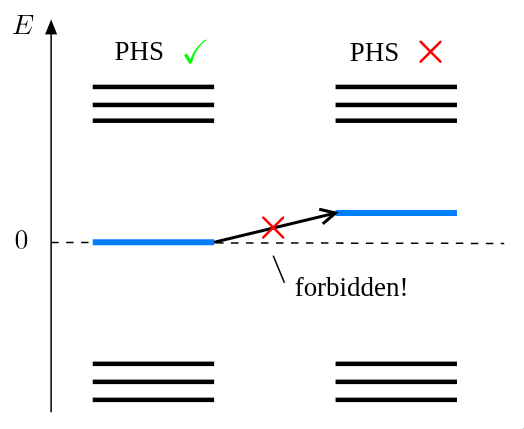
\includegraphics[width=0.5\textwidth]{../External_Figs/gs_symmetry.png}%
  \caption{Energy spectrum showing how the energy eigenvalues of the system must be symmetric around zero energy due to particle-hole symmetry \textcolor{red}{CITATION}Topocondmat.org (Bulk edge correspondence in Kitaev chains)}
  \label{fig:gs_symmetry}
\end{figure}
\newpage
\subsubsection{Local distinguishability}
A property of the Kitaev chain in its topological phase is that measurements done locally cannot reveal if the system is in its odd or even ground state. Meaning the two ground states are locally indistinguishable. In order to quantify this property, we will define the local distinguishability parameter LD as:
$$
\text{LD} = \frac{1}{N} \sum_{j=1}^{N} || ρ_j^o - ρ_j^e || = \frac{1}{N} \sum_{j=1}^{N} || δ ρ_j ||
$$
\textcolor{red}{CITATION}[Majorana bound states in chains
of interacting quantum dots Viktor ].\\Here, $ρ_j^{o/e}$ are the reduced density matrices of site $j$ for the odd and even parity ground states, respectively. The norm $|| \cdot ||$ is the trace norm, which measures the difference between the two local states. The LD parameter quantifies how distinguishable the two ground states are when only local measurements are considered. A value of LD close to zero indicates that the two states are nearly indistinguishable locally, which is a hallmark of Majorana modes. Conversely, a value close to one indicates that the states can be easily distinguished by local measurements, suggesting the absence of Majorana modes.\\
\subsubsection{Majorana polarization}
In interaction Kitaev chains with finite magnetic fields, there are no ideal Majorana sweet spots, as the presence of the other spin species introduces corrections to the simple picture of Majorana modes. However, sweet spots with very good Majorana localization and close to degenerate ground states with even and odd parity can still appear in the system. To quantify how close we are to an ideal Majorana mode, we can use the Majorana polarization (MP) metric. The MP is a measure of how well the Majorana modes are localized at the ends of the chain and how closely they resemble ideal Majorana fermions. The MP is defined as:
$$
M_α = \frac{W_α^2 - Z_α^2}{W_α^2 + Z_α^2}
$$
where,
$$
W_α = ∑_{σ} \bra{o} c_{ασ} + c_{ασ}^{†} \ket{e}, \quad Z_α = i ∑_{σ} \bra{o} c_{ασ} - c_{ασ}^{†} \ket{e}
$$
Here, $α$ denotes the site index (left or right dot), $σ$ is the spin index, and $\ket{o}$ and $\ket{e}$ are the odd and even parity ground states, respectively. In an ideal sweet spot where two Majoranas are perfectly localized on the left and right dots, the MP values would be $M_L = -M_R = ± 1$. \textcolor{red}{CITATION}[Chap3 qtech].\\
\subsubsection{Charge expectation and non-locality}
The last measurable property we will discuss is the charge expectation value of the ground states. This id measured by taking the expectation values of the number operators in the odd and even ground states:
$$
\bra{e}n_{L(R)} \ket{e}, \quad \bra{o}n_{L(R)} \ket{o}
$$
where $n_{L(R)}$ is the number operator for the left (right) dot. In the ideal case, these expectation values should be equal for both ground states. This is because, if the difference is zero, the two ground states share the same local charge distribution, making them locally indistinguishable. 




















\section{Analytical and Numerical Investigation of PMMs}
Present my work and demonstrate how to apply theory to a concrete problem.\par
\subsection{Single particle model:}
\subsubsection{The Model Hamiltonian:} Present the minimal Hamiltonian for the QD-SC-QD system that i have in my notes note section 5.2.2, for instance Eq 3.54 from chap3.pdf. Define all the terms clearly. This will be the Hamiltonian I use.\par
$$  
  H = \begin{pmatrix}
    ϵ_L & t & 0 & Δ \\
    t & ϵ_R & -Δ & 0 \\
    0 & -Δ & -ϵ_L & -t \\
    Δ & 0 & -t & -ϵ_R
  \end{pmatrix}
$$
Where $ϵ_L$ and $ϵ_R$ are the energy levels of the left and right dots, $t$ is the elastic cotunneling amplitude, and $Δ$ is the CAR amplitude. The basis is $(d_L, d_R, d_L^{†}, d_R^{†})$, called the Nambu basis. The operators $d_L^{†}$ and $d_R^{†}$ create an electron in the left and right dot, respectively.\par

\subsubsection{Analytical Work - Finding the Sweet Spot:} Solve the Hamiltonian for the simplest case: two indentical dots with their energy levels at zero ($ϵ_L = ϵ_R = 0$). I can write the $4x4$ matrix in the Nambu basis $Ψ^{†}= (d_L, d_R, d_L^{†}, d_R^{†})$. Show analytically that the condition for having two zero energy solutions (the Majoranas) is at $|t| = |Δ|$.This proves i understand the sweet spot.\par

Solving the eigenvalue problem $HΨ = EΨ$ gives the characteristic polynomial:
$$
\text{det}(H - EI) = \begin{pmatrix}
    ϵ_L-E & t & 0 & Δ \\
    t & ϵ_R-E & -Δ & 0 \\
    0 & -Δ & -ϵ_L-E & -t \\
    Δ & 0 & -t & -ϵ_R-E
\end{pmatrix} =0
$$
$$
= E⁴ -E²a + b=0
$$
where
$$
a = ϵ_L² + ϵ_R² + 2(t² + Δ²)
$$
and 
$$
b = (t² - ϵ_Lϵ_R - Δ²)² 
$$
The quadratic formula for $E²$ gives:
$$
E² = \frac{a ± \sqrt{a² - 4b}}{2}
$$
The discriminant simplifies to:
$$
a² - 4b = [(ϵ_L+ϵ_R)² + 4t²][(ϵ_L - ϵ_R)² + 4Δ²]
$$
and the eigenvalues are $±\sqrt{E²}$. For zero energy solutions, we need $b=0$, which requires:
$$
t² - ϵ_Lϵ_R - Δ² = 0
$$
At $ϵ_L = ϵ_R = 0$, this reduces to the sweet spot condition:
$$|t| = |Δ|$$
With the conditions we obtained from setting $b=0$, $a$ becomes $2(t² + Δ²)=4t²$.\\
With $b=0$, the quadratic formula simplifies to $E²(E²-a)=0$, giving us two solutions:
$$
E² = 0 \quad E² = a = 4t²
$$
Therefore the four eigenvalues are:
$$
E = \{0, 0, 2|t|, -2|t|\}
$$
These eigenvalues have corresponding eigenvectors. \\
For $E=0$, the eigenvectors are:
$$
v_1 =  \begin{pmatrix} 1 \\ 0 \\ 1 \\ 0 \end{pmatrix}, \quad v_2 = \begin{pmatrix} 0 \\ 1 \\ 0 \\ -1 \end{pmatrix}
$$
and for $E=2|t|$, the eigenvectors are:
$$
v_3 =  \begin{pmatrix} -1 \\ 1 \\ 1 \\ 1 \end{pmatrix}, \quad v_4 = \begin{pmatrix} 1\\ 1 \\ -1 \\ 1\end{pmatrix}
$$
The zero-mode eigenvectors $v_1$ and $v_2$ correspond to the Majorana operators. The two zero-energy eigenvectors,
$v_1$ and $v_2$, represent states that are equal superpositions of particle and hole operators on a single dot. In operator form, they correspond to self-conjugate combinations:
$$
γ_1 ∝ d_L + d_L^{†}, \quad γ_2 ∝ d_R - d_R^{†}
$$
which satisfy the Majorana condition $γ = γ^{†}$. These are the Poor Man's Majorana modes. They are spatially separated zero modes, localized entirely on the left and right dots at the sweet spot $|t| = |Δ|$ and $ϵ_L = ϵ_R = 0$.\\
Their degeneracy at zero energy encodes the nonlocal fermionic parity of the two-dot system, which is the resource we ultimately want for quantum information.\\ 
By contrast, the finite-energy solutions 
$$E = ±2|t|, \quad v_3 ∝ (-1, 1, 1, 1)^T, \quad v_4 ∝ (1, 1, -1, 1)^T$$
are delocalized Bogoliubov quasiparticles. They form the first excited states above the ground state and define the energy gap protecting the Majorana subspace. Physically, this gap is crucial: as long as it remains finite, the Majorana modes cannot hybridize with bulk excitations, and the zero-energy subspace is robust against small perturbations. 

\subsubsection{Numerical Simulations - Visualize the Emergence of Majoranas:} Build and diagonalize the Hamiltonian numerically. Band Structure: Plot the two lowest positive energy eigenvalues as a function of a dot's energy $ϵ_L$ (keeping $ϵ_R = 0$) and $t = Δ$. Reproduce the plot from Fig 3.5a in chap3.pdf showing two states remaining at zero energy, showcasing the symmetry. Wavefunctions: At the sweet spot ($t = Δ$ and $ϵ_L = ϵ_R = 0$), find the eigenvectors for the two zero-mode energy states. Plot the magnitude of the components. I should be able to see that one zero mode is localized entirely on the left dot and the other is entirely on the right dot, confirming they are spatially separated Majoranas.\par
\subsubsection{Numerical Work - Probing Protection and Robustness:} Detuning $t$ and $Δ$: Vary $t$ and $Δ$ away from the sweet spot. Plot the lowest energy eigenvalue as I varyt he ratio $\frac{t}{Δ}$ away from 1. This will show that the zero-energy states immediately split and acquire a finite energy gap, demonstrating their lack of full topological protection. Detuning Dot Energies: Vary $ϵ_L$ and $ϵ_R$ away from zero while keeping $t = Δ$. The degeneracy should be lifted quadratically. My results here should quantify the robustness of the PMMs to local perturbations. I can conclude that while they are not fully protected like in a true topological system, the degeneracy is protected against certain local perturbations to first order.\par

\subsection{Many-body model:} (Including the Coulomb interaction $U$)
\subsubsection{The Model Hamiltonian:} Present the many-body Hamiltonian for the QD-SC-QD system, including the Coulomb interaction term $U$. Define all the terms clearly. This will be the Hamiltonian I use.\par
We have to leave the BdG formalism and work in the many-body basis. This is because the BdG formalism is a mean-field, single-particle approach that cannot capture electron-electron interactions like the Coulomb repulsion $U$. The interaction term we use in order to describe the non-local Coulomb interaction betweem the PMMs is: $H_U=U_{LR}n_Ln_R$, where $n_{α}=d_{α}^{†}d_{α}$ is the number operator for dot $α$.\\
The full Hamiltonian for the QD-SC-QD system with Coulomb interaction is:
$$
H = ∑_{α=L,R} ϵ_{α} d_{α}^{†}d_{α} + t (d_L^{†} d_R + d_R^{†} d_L) + Δ (d_R d_L + d_L^{†} d_R^{†})  + U_{LR} n_L n_R
$$
where $ϵ_{α}$ are the energy levels of the left and right dots, $t$ is the elastic cotunneling amplitude, $Δ$ is the CAR amplitude, and $U_{LR}$ is the non-local Coulomb interaction between electrons on the two dots. The basis states for the two-dot system are: $|0,0⟩$, $|1,0⟩$, $|0,1⟩$, $|1,1⟩$, where $|n_L,n_R⟩$ indicates the occupation of the left and right dots.\par
We can now proceed to construct the Hamiltonian matrix in this many-body basis, where it becomes:
$$
H = \begin{pmatrix}
0 & 0 & 0 & Δ \\
0 & ϵ_R & t & 0 \\
0 & t & ϵ_L & 0 \\
Δ & 0 & 0 & ϵ_L + ϵ_R + U_{LR}
\end{pmatrix}
$$
\subsubsection{Analytical Work - Exploring the many body Hamiltonian:} 
The many-body Hamiltonian above is written in the basis order:
$$ |0,0⟩, |0,1⟩, |1,0⟩, |1,1⟩ $$
Due to order and practicality, we can try to rewrite the Hamiltonian in a block-diagonal manner. To do so, we can first investigat the matrix elements we have. The even sector is spanned by the states $|0,0⟩$ and $|1,1⟩$, which correspond to the matrix elements $H_{11}, H_{14}, H_{41}, H_{44}$. The odd sector is spanned by the states $|0,1⟩$ and $|1,0⟩$, which correspond to the matrix elements $H_{22}, H_{23}, H_{32}, H_{33}$.\\
If we reorder the basis as [even, odd] = $[|0,0⟩, |1,1⟩, |0,1⟩, |1,0⟩]$, we obtain:
$$
H = \begin{pmatrix}
0 & Δ & 0 & 0 \\
Δ & ϵ_L + ϵ_R + U_{LR} & 0 & 0 \\
0 & 0 & ϵ_R & t \\
0 & 0 & t & ϵ_L
\end{pmatrix}
$$
This is now block-diagonal, with the even sector in the top-left $2x2$ block and the odd sector in the bottom-right $2x2$ block.\\
In other words, we have:
$$
H = \begin{pmatrix}
H_{even} & 0 \\
0 & H_{odd}
\end{pmatrix}
$$
with:
$$
H_{even} = \begin{pmatrix}
0 & Δ \\
Δ & ϵ_L + ϵ_R + U_{LR}
\end{pmatrix}, \quad
H_{odd} = \begin{pmatrix}
ϵ_R & t \\
t & ϵ_L
\end{pmatrix}
$$
Our next step is to find an expression for the eigenvalues of each sector. For simplicity we will call $S = ϵ_L + ϵ_R + U_{LR}$. Starting with the even sector, we solve the characteristic polynomial:
$$
\text{det}(H_{even} - EI) = \begin{pmatrix}
    -E & Δ \\
    Δ & S - E
\end{pmatrix} =0
$$
This gives us the quadratic equation:
$$
E² - SE + (Δ²) = 0
$$
Using the quadratic formula, we find the eigenvalues for the even sector:
$$E_{even} = \frac{S ± \sqrt{S² + 4Δ²}}{2} = \frac{ϵ_L + ϵ_R + U_{LR} ± \sqrt{(ϵ_L + ϵ_R + U_{LR})² + 4Δ²}}{2}$$
Next, we solve the characteristic polynomial for the odd sector:
$$
\text{det}(H_{odd} - EI) = \begin{pmatrix}
    ϵ_R - E & t \\
    t & ϵ_L - E
\end{pmatrix} =0
$$
This gives us the quadratic equation:
$$(ϵ_R-E)(ϵ_L - E)  - t² = 0$$
$$E² -(ϵ_R-ϵ_L)E + ϵ_R ϵ_L - t² = 0$$
Using the quadratic formula, we find the eigenvalues for the odd sector:
$$E_{odd} = \frac{(ϵ_L + ϵ_R) ± \sqrt{(ϵ_L - ϵ_R)² + 4t²}}{2}$$

\subsubsection{Analytical Work - Finding the Conditions for a Many-body Sweet Spot:}
To find the conditions for having two degenerate ground states (one from each sector), we set the lowest eigenvalue from each sector equal to each other:
$$E_{\text{even,min}} = E_{\text{odd,min}}$$


\subsubsection{How Majorana like?}
This section is per now just notes: Fill in the blanks along the way.\\
$\ket{e}, \ket{o}$ are the ground states of the even and odd sectors, respectively. Find them:\\\\
Three (four) things to look for to see if we found topologically protected Majoranas:\\
1) Degeneracy of ground states: We need $E_{even,min} = E_{odd,min}\quad  δE=0$\\
2-3) With the number operators $n_L$ and $n_R$, we can calculate the expectation values $\bra{e}n_{L(R)}\ket{e}$ and $\bra{o}n_{L(R)}\ket{o}$. The difference in occupation between the two ground states on each dot should be minimal, ideally zero. This indicates that the Majorana modes are non-local and do not localize charge on either dot.\\
4) Find the Majorana polarization $MP = 1$

\section{Discussion and Conclusion}
\subsection{Synthesize my Findings:} Summarize what we learned from the calculations. " The analysis confirmed that zero-energy Majorana modes emerge under fine-tuned conditions... Numerical simulations revealed that this degeneracy is fragile and splits when deviating from the sweet spot, quantifying the limited protection of PMMs."\par
\subsection{Connect to Broader Context:} Briefly discuss how the properties you explored (the energy splitting, wavefunction overlap) would affect potential braiding operations (note section 5.2.3) and what this means for using PMMs in quantum computing.\par
\subsection{Future Directions:} Suggest next steps for a full thesis. This include modeling disorder, investigating longer chains (three or more dots), or numerically simulate braiding protocol.



\end{document}











